% !TEX root = ../Dokumentation.tex
\subsection{Fahrbahnerkennung}
\textbf{Umsetzung}\\[0.2cm]
Die Fahrbahnerkennung ist primär mittels Kamera realisiert. Es wird jeweils das aktuelle Bild von der Klasse \code{PictureCreator} entnommen, mit OpenCV in Graustufen umgewandelt und anschliessend an die Kantenerkennung weitergegeben. Für die Kanten wird eine eigene Matrix erstellt, vorgelegt mit dem Graustufenwert 0. Die Kantenerkennung basiert auf der Differentialrechnung und betrachtet vom aktuellen Pixel aus in $x$ (Spalte) und $y$ (Zeile) den Graustufenwert des nächsten Pixels und des vorherigen Pixels.
$z = f(x,y) = \text{ Graustufen des Pixels }0 \leq z \leq 255$\\
\[
\frac{\partial{z}}{\partial{x}}=\frac{f(x+\Delta{x})-f(x-\Delta{x})}{2\Delta{x}} = \frac{f(x+1)-f(x-1)}{2}
\]
\[
\frac{\partial{z}}{\partial{y}}=\frac{f(y+\Delta{x})-f(y-\Delta{y})}{2\Delta{y}} = \frac{f(y+1)-f(y-1)}{2}
\]
\[
\nabla f(x,y) = \begin{bmatrix}
\frac{\partial{z}}{\partial{x}}\\
\frac{\partial{z}}{\partial{y}}
\end{bmatrix}
\]
\[
\lVert\nabla f(x,y)\rVert = \sqrt{\Biggl(\frac{\partial{z}}{\partial{x}}\Biggr)^2 + \Biggl(\frac{\partial{z}}{\partial{y}}\Biggr)^2}
\]
Übersteigt die Änderung der Graustufe den vorgegebenen Schwellwert wird eine Kante erkannt, an die entsprechende Pixelposition der Zielmatrix wird der Wert 255 geschrieben, ansonsten nicht. Mit der Festgelegten Kameraposition beschränkt sich die Fahrbahnerkennung auf die untere Bildhälfte. Damit werden störende Effekte in der Umgebung vermieden (Abbildung: \ref{fig:edges}). 
\begin{figure}[H]%Position festigen
\centering
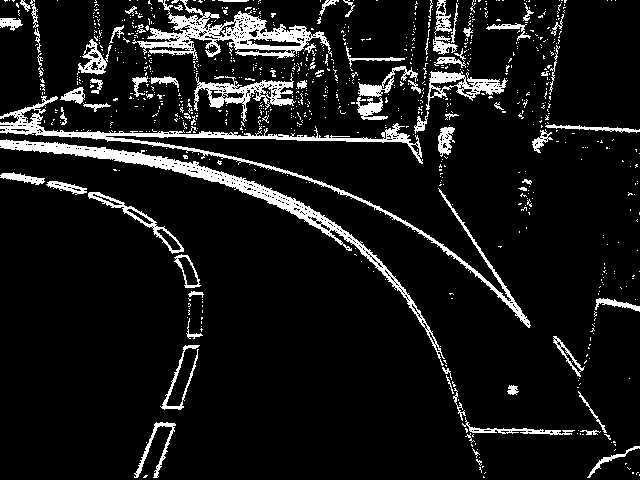
\includegraphics[width=0.6\textwidth]{03_Loesungskonzept/pictures/Kantengrafik.png}
\caption{Bild nach Kantenerkennung}
\label{fig:edges}
\end{figure}
Im Anschluss an die Kantendetektion folgt eine Linienerkennung mittels Hough-Transformation. Dabei werden alle Linien vorgefiltert, die nicht zur Fahrbahn gehören können. Dies wird anhand der Steigung ermittelt. Die gültigen Linien werden im Anschluss harmonisiert, das Heisst ihr Start- und Endpunkt wird so angepasst, dass 
immer der Startpunkt in $y$-Richtung am Maximum liegt. Weiter wird die Linie auf die untere Bildkante verlängert. Im Anschluss werden nur die innersten Linien behalten und zur Berechnung der Fahrtrichtung weitergegeben (Abbildung: \ref{fig:routeLimits}). Zur optischen Hilfe ist die Bildmitte markiert um die ermittelten Abstände visuell prüfen zu können.
\begin{figure}[H]%Position festigen
\centering
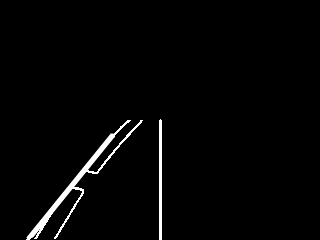
\includegraphics[width=0.7\textwidth]{03_Loesungskonzept/pictures/Fahrbahnlinien.png}
\caption{Eingetragene Fahrbahngrenze}
\label{fig:routeLimits}
\end{figure}
Um die Fahrtrichtung zu prüfen werden nun die ermittelten Fahrbahnlinien ausgewertet. Wenn beide Fahrbahnseiten erkannt werden, wird der Mittelwert aus beiden genutzt ansonsten jeweils die vorhandene Seite. Die Auswertung erfolgt nach folgenden Schritten:
\begin{enumerate}
\item Verzerrungskorrektur rechnen: Da schräg auf die Fahrbahn geschaut wird ist die Fahrbahn nicht parallel sondern entsprechend gegen die Bildrichtung zusammenlaufend. Dies wird für die Abstandsermittlung berücksichtigt. Der Neigungswinkel der Kamera ist so gewählt, dass die Korrektur mit folgender, einfacher Formel berechnet werden kann:
\[
D = \frac{y}{2} + 40 
\]
Wobei $D$ der Solldistanz und $y$ der höheren Bildzeile der Linie entspricht. Diese Formel ist nur gültig, da bei gerader Fahrbahn die Differenz zwischen oberer und unterer Distanz der Fahrbahnlinien exakt der Hälfte der Bildhöhe entspricht (Abbildung: \ref{fig:routeCorr}).
\item Abstand mit Sollwert vergleichen und die Differenz ermitteln.
\item Den Winkel der Korrektur berechnen. Die Kamera schaut 200mm vor die Mitte der Vorderachse, was 160 Bildpixel entspricht.
\item Der ermittelte Korrekturwinkel wird an den PID-Regler weitergegeben.
\end{enumerate}
\begin{figure}[H]%Position festigen
\centering
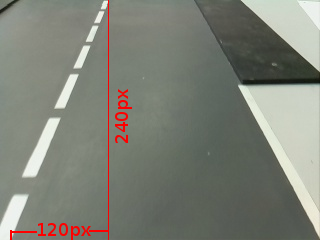
\includegraphics[width=0.7\textwidth]{03_Loesungskonzept/pictures/Verzerrung.png}
\caption{Verzerrung des Bildes}
\label{fig:routeCorr}
\end{figure}
Zugleich der Fahrbahnermittlung wird für jedes Bild die Steigung der Fahrbahnkanten überwacht. Unterschreiten diese die Mindestgrenze, wird eine Kurve erkannt und die Kamera auf einen Winkel von 30° eingelenkt. Entprechend wird die Solldistanz um den entsprechenden Pixelwert aus der Mitte versetzt um die veränderte Perspektive auszugleichen. Uberschreitet die Steigung der Fahrbahnlinien die Obergrenze wird die Kamera wieder auf die gerade Position zurückgeschwenkt.\\
Um zu Beginn ein Einlenken der Kamera zu verhindern wird diese Funktion erst nach einer gewissen Anzahl verarbeiteter Bilder aktiviert. Der Wert kann in der Konfigurationsdatei festgelegt werden.
\newpage
\textbf{Komponentenbeschrieb}
\begin{figure}[H]%Position festigen
\centering
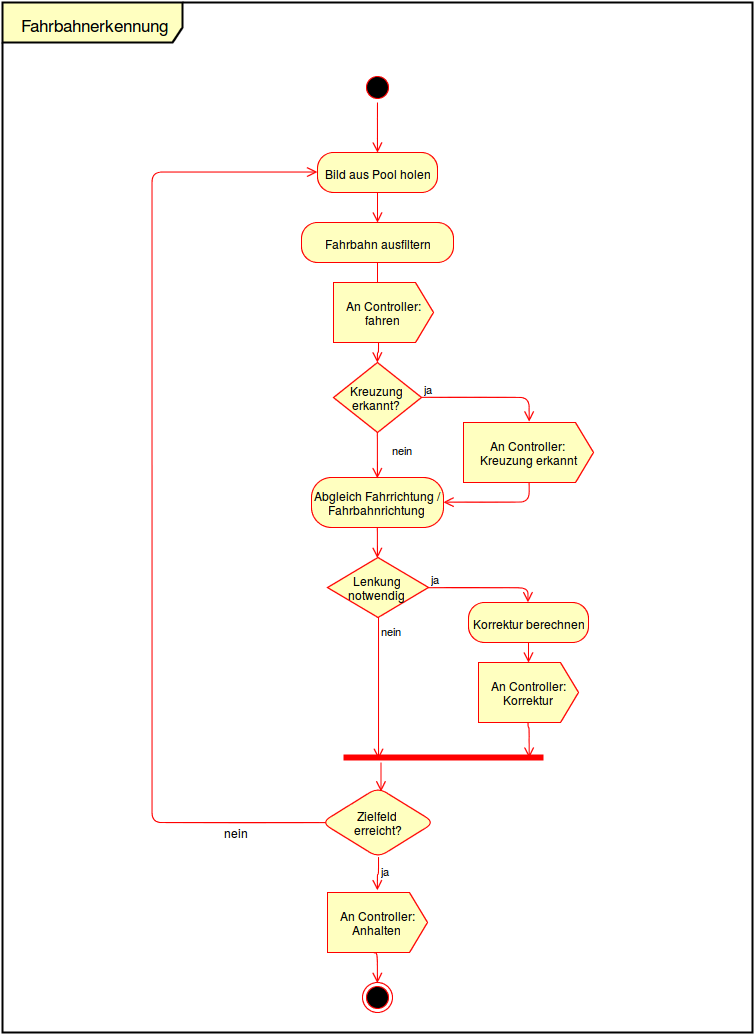
\includegraphics[width=0.7\textwidth]{03_Loesungskonzept/pictures/Fahrbahnerkennung.png}
\caption{Aktivitätendiagramm Fahrbahnerkennung}
\label{fig:activityRoute}
\end{figure}
Die Fahrbahnkanten werden im Anschluss anhand der ermittelten Werte gesucht. Ist eine Kante in der Nähe der ermittelten Fahrbahn, wird sie behalten, ansonsten entfernt. Der Grenzwert muss noch genau ermittelt werden.\\
Die Parameter für die Regelung werden mit folgender Formel ermittelt:
\[
G_R = K_p\left(1 + \frac{1}{T_{n^S} + T_{v^S}}\right)
\]
Danach werden die ermittelten Werte in die Korrekturformel eingesetzt:
\[
y = K_{PR}\left(e + \frac{1}{T_n}\int{edt} + T_v\dot{e}\right)
\]
wobei $y$ dem zu korrigierenden Winkelwert in Grad entspricht. Die Parameter $T_v$, $T_n$ und $K_{PR}$ müssen für die Feineinstellung justierbar sein. Dies soll für die Debugphase über eine auf dem Notebook betriebene Software geschehen.
\newpage
\underline{\textbf{Fahrbahnerkennung Unterstützung}}\\[0.2cm]
Unterstützend zur Kameraauswertung hat die Steuerung noch eine weitere Angabe zur Verfügung. Dies ist die gemessene Distanz des Fahrzeuges zum Gehsteig. Dies wird über den Flexsensor realisiert. Wie in der Dokumentation von Pren1 erläutert, ändert der Flexsensor seinen Widerstandswert je nachdem wie fest der Sensor gebogen ist. Der Widerstandswert wird über den Analog-Digitalwandler in dem Mikrocontroller eingelesen. Beim einlesen diese Wertes wurde festgestellt, dass dieser relativ grosses Rauschen enthält. Verursacht wurde diese Rauschen hauptsächlich von der 5V Speisung. Diese enthält selbst gewisse Störungen, welche nachher den Messwert beeinflussen. Gelöst wurde diese Problem, indem zusätzlich zum Flexsensorwert auch ein Spannungswert relativ zur Speisung eingelesen wird. Aus diesen beiden Messwerte kann das differentielle Signal berechnet werden, aus dem die Störungen am 5V Netz weniger Einfluss haben. Mit dem bereinigtem Signal kann nun der ungefähre Abstand zum Gehsteig berechnet werden. Dies geschieht über eine lineare Funktion. Die Umrechnung vom Widerstandswert zum Abstand stimmt somit nicht sehr genau, sollte aber als Zusatzinformation so reichen.%Todo Führ Bild vom montiertem Flexsensor ein.
\\[0.2cm]
\textbf{Vergleich Konzept und Umsetzung}\\[0.2cm]
Das Konzept wurde für den Flexsensor nicht verändert. Dieser war immer als Hilfswert gedacht und dies wurde nun auch so implementiert. Angepasst wurde lediglich die Messmethode, welche nun differentiell geschieht.